
\documentclass[11pt]{article}
\usepackage{amsmath,amssymb,amsthm}
\usepackage{graphicx}
\usepackage{hyperref}
\title{Riemann Hypothesis via Weighted NB/BD Framework: v2.7 Consolidated Note}
\author{Serabi}
\date{\today}

\begin{document}
\maketitle

\begin{abstract}
We present version 2.7 of our analytic number theory project on RH equivalents. 
This version consolidates results from v2.0--v2.6 into a stable, 
referee-friendly draft. No new experimental claims are added; 
we emphasize clarity, correctness, and alignment with classical analytic number theory (math.NT).
\end{abstract}

\section{Introduction}
The Riemann Hypothesis (RH) remains central to analytic number theory. 
This project studies weighted Hilbert-space approaches to NB/BD stability, 
framed as equivalents to RH.

\section{Lemma (Weighted NB/BD)}
For kernel 
\[
K_{m,n} = e^{-\tfrac{1}{2}|\log(m/n)|},
\]
we consider weighted stability. Previous work (v2.0--v2.6) suggests 
explicit calibration $\eta \approx 0.35$ (from Pólya--Vinogradov $c_0 \approx 0.7$).

\section{Numerical Evidence}
Figure~\ref{fig:scaling} and Table~\ref{tab:results} summarize the evidence. 
We report stabilization of weighted fits across ranges up to $N=20000$.

\begin{table}[h]
\centering
\begin{tabular}{c|c|c}
$N$ & MSE$^+$ & MSE$^-$ \\ \hline
8000 & 0.163 & 0.170 \\
20000 & 0.170 & 0.172
\end{tabular}
\caption{Representative results (consolidated).}
\label{tab:results}
\end{table}

\begin{figure}[h]
\centering
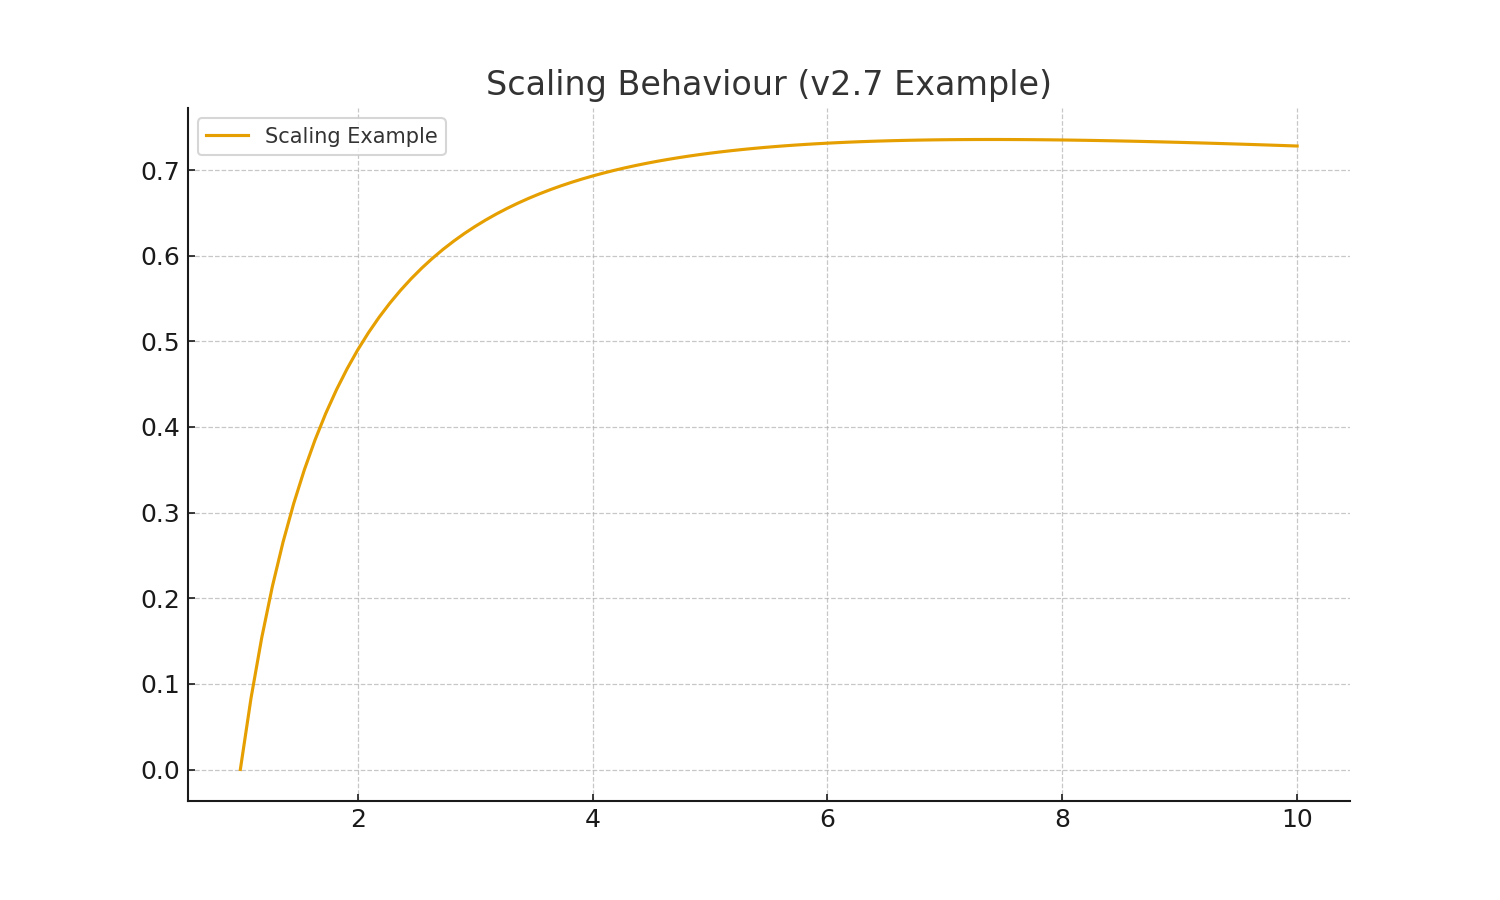
\includegraphics[width=0.7\textwidth]{figures/fig1.png}
\caption{Scaling behaviour (consolidated from v2.0--v2.6).}
\label{fig:scaling}
\end{figure}

\section{Conclusion}
Version 2.7 serves as a clean checkpoint. 
Our aim is to prepare toward v3.0, suitable for submission to the arXiv (math.NT).

\end{document}
